\documentclass[tikz,border=3mm]{standalone}
\usepackage{pgfplots}
\pgfplotsset{compat=1.17}
\begin{document}
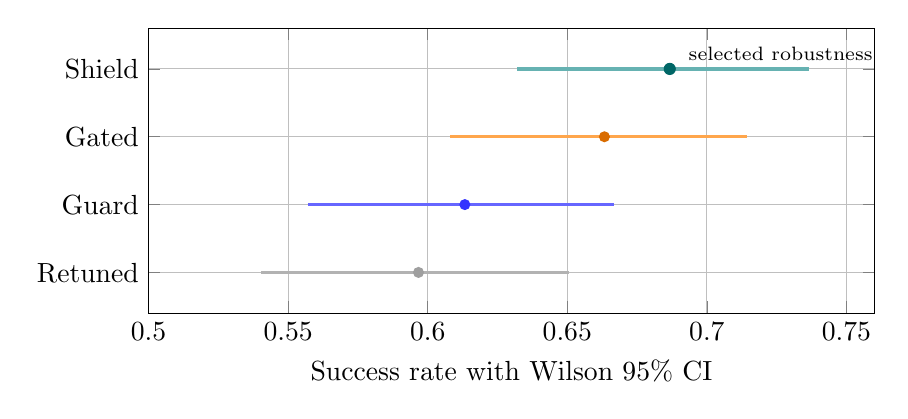
\begin{tikzpicture}
\begin{axis}[width=10.8cm,height=5.2cm,xmin=0.50,xmax=0.76,ymin=0.4,ymax=4.6, xlabel={Success rate with Wilson 95\% CI}, ytick={1,2,3,4}, yticklabels={Retuned,Guard,Gated,Shield}, grid=major]
\draw[line width=1.2pt, color=gray!60] (axis cs:0.5403,1) -- (axis cs:0.6506,1);
\fill[gray!75] (axis cs:0.5967,1) circle (2.0pt);
\draw[line width=1.2pt, color=blue!60] (axis cs:0.5571,2) -- (axis cs:0.6667,2);
\fill[blue!80] (axis cs:0.6133,2) circle (2.0pt);
\draw[line width=1.2pt, color=orange!70] (axis cs:0.6081,3) -- (axis cs:0.7144,3);
\fill[orange!85!black] (axis cs:0.6633,3) circle (2.0pt);
\draw[line width=1.2pt, color=teal!60] (axis cs:0.6321,4) -- (axis cs:0.7365,4);
\fill[teal!80!black] (axis cs:0.6867,4) circle (2.2pt);
\node[font=\scriptsize,anchor=west] at (axis cs:0.690,4.22) {selected robustness mode};
\end{axis}
\end{tikzpicture}
\end{document}
